\documentclass[apj]{emulateapj}
\usepackage{color}
\usepackage{natbib}
\bibliographystyle{apj}

\newcommand{\vdag}{(v)^\dagger}
\newcommand{\myemail}{eogorma@tcd.ie}

\shorttitle{The CO Shells of Betelgeuse}
\shortauthors{O'Gorman et al.}

\begin{document}

\title{CARMA CO(\textit{J} = 2-1) Observations of the Circumstellar \\ Envelope of Betelgeuse}

\author{Eamon O'Gorman and Graham M. Harper}
\affil{School of Physics, Trinity College Dublin, Dublin 2, Ireland}
\email{eogorma@tcd.ie}
\email{graham.harper@tcd.ie}

\author{Joanna M. Brown}
\affil{Harvard-Smithsonian Center for Astrophysics, 60 Garden Street, \\ MS-78, Cambridge, MA 02138, USA}
\email{joannabrown@cfa.harvard.edu}

\author{Alexander Brown}
\affil{Center for Astrophysics and Space Astronomy, University of Colorado, \\ 389 UCB, Boulder, CO 80309, USA}
\email{alexander.brown@colorado.edu}

\author{Seth Redfield}
\affil{Astronomy Department, Van Vleck Observatory, Wesleyan University, \\ Middletown, CT 06459, USA}
\email{sredfield@wesleyan.edu}

\and

\author{Miguel A. Requena-Torres}
\affil{Max-Planck-Institut für Radioastronomie, Auf dem Hügel 69, \\ 53121 Bonn, Germany}
\email{mrequena@mpifr-bonn.mpg.de}

\begin{abstract}
We report radio interferometric observations of the $\rm{{}^{12}}$C$\rm{{}^{16}}O$ 1.3 mm J=2-1 emission line in the circumstellar envelope of the M supergiant $\alpha$ Ori.  Observations were made with the Combined Array for Research in Millimeter-wave Astronomy (CARMA) interferometer in the C, D, and E antenna configurations. We obtain excellent  uv-coverage (5 - 280 k$\lambda$) by combining data from all three configurations allowing us to trace spatial scales as small as $0.9\arcsec$ over a $32\arcsec$ field of view. The high spatial resolution C configuration maps show that the inner S1 shell has asymmetric outflow velocities ranging from -9.0 km s${}^{-1}$ to +10.6 km s${}^{-1}$ with respect to the stellar rest frame. We find little evidence  for the outer S2 shell in this configuration probably because the majority of this emission has been spatially-filtered (resolved out) by the array. The S2 shell appears as an extra blueshifted emission component in the D and E configuration maps between -11.0 km s${}^{-1}$  and -16.0 km s${}^{-1}$ and we detect it between +10.6 km s${}^{-1}$ and + 13.2 km s${}^{-1}$ in the redshifted portion of the line profile. The S2 shell's outflow velocity is found to be in good agreement with high resolution optical spectroscopy of KI. A discrete off-source emission feature is detected at 5$\arcsec$ S-W of  $\alpha$ Ori in all D configuration maps. We image both shells in the multi-configuration maps (all configurations) and see the formation of the classical ring structure for the S2 shell as we sample the line across velocities. We assign an outer radius of 5$\arcsec$ to S1 and propose that S2 extends beyond CARMA's field of view (32$\arcsec$ at 1.3 mm) out to a radius of 17$\arcsec$ which is larger than recent single dish observations have indicated. 
\end{abstract}

\keywords{circumstellar matter --- Stars: individual: ($\rm{\alpha}$ Ori) --- Stars: late-type --- Stars: massive --- supergiants --- Radio lines: stars}

\section{INTRODUCTION}

\begin{center}
\begin{deluxetable*}{cccccc}
\tabletypesize{\scriptsize}
%\tablecolumns{6} 
\tablewidth{0pt} 
\tablecaption{CARMA Observations}
\tablehead{\colhead{Observation}		                                &
                 \colhead{Configuration}				&
          	\colhead{Time on Source}	      			&
	\colhead{Flux}			    	     	&
           	\colhead{Phase}                                       		&
	\colhead{Image Cube\tablenotemark{a}}		\\
	\colhead{Date}					&
           	\colhead{}                				& 
	\colhead{(hr)}                                          		& 
	\colhead{Calibrator}                                          		& 
	\colhead{Calibrators}                                          		&
	\colhead{Dynamic Range\tablenotemark{b}}		}
\startdata
2007 Jun 18 	& D & 0.9 & 0530+135	& 0530+135, 0532+075 	&  22.8 \\
2007 Jun 21 	& D & 3.0 & 0530+135	& 0530+135, 0532+075 	&  22.7 \\
2007 Jun 24 	& D & 2.1 & 0530+135	& 0530+135, 0532+075 	&  26.1 \\
2007 Jun 25 	& D & 2.4 & 0530+135	& 0530+135, 0532+075 	&  30.2 \\
2009 Jul 07	& E & 3.2 & 3C120 		& 3C120, 0532+075	& 30.1 \\
2009 Nov 05	& C & 1.2 & 3C120 		& 3C120, 0532+075 	& 17.3 \\
2009 Nov 09 	& C & 3.0 & 3C120 		& 3C120, 0532+075 	& 27.2 \\
2009 Nov 15	& C & 1.0 & 3C120 		& 3C120, 0532+075 	& 17.8 \\
2009 Nov 16	& C & 3.2 & 3C120 		& 3C120, 0532+075 	& 32.0  \\
All		& C & 8.4	& \nodata 	& \nodata 		& 43.8 \\
All 		& D & 8.4 & \nodata 	& \nodata 		& 31.9 \\
All 		& Multi-configuration & 20.0 & \nodata & \nodata 	& 52.3 
\enddata
\tablenotetext{a}{Low spectral resolution (i.e. channel width of 1.3 km s$\rm{{}^{-1}}$).}
\tablenotetext{b}{The peak emission of the image cube divided by the root mean square of the residual image.}
\label{tab:tab1}
\end{deluxetable*}
\end{center}

The circumstellar envelope (CSE) of Betelgeuse ($\alpha$ Orionis [M2 Iab]) is a proving ground for ideas and theories of mass loss from oxygen-rich M supergiants. Currently it is losing mass at a respectable rate $\sim 3\times 10^{-6} \ M{}_{\odot}$ yr${}^{-1}$ \citep{1986ApJ...306..605G, 1994ApJ...424L.127H,harper_2001}, as it has been in the past $\sim$ 1000 yr. Most of the optically thin silicate dust lies beyond $\sim 30$ stellar radii \citep{1994AJ....107.1469D} and dust is, therefore, unlikely to be responsible for the bulk mass loss as is the case in M-type supergiants. This raises the important point that if the mass loss from Betelgeuse is not a result of dust then perhaps the same mechanisms that are responsible might also be active in the more dusty later M-type supergiants. 

\cite{1984ApJ...284..238H} constructed a magnetic WKB Alfv\'{e}n wave-driven model for Betelgeuse's chromosphere and wind that reproduced reasonably well the observed chromospheric emission fluxes and mass loss rate. However, multi-wavelength centimeter continuum radio observations made with the Very Large Array (VLA) by \cite{1998Natur.392..575L} revealed that the atmosphere was much cooler than the Alfv\'{e}n wave-driven model predicted \citep{harper_2001}. Although  new nonlinear Alfv\'{e}n wave models have been computed by \cite{2000ApJ...528..965A} there are currently no theoretical models that make specific predictions for {\em both} the dynamic and thermodynamic state of the mass outflow. 

Radiation pressure on atoms and molecules is another potential contributing candidate for mass loss mechanism and so spatial and dynamical studies of molecules are a fruitful line of investigation, especially in relation to eventual formation of dust. The study of CO molecules in the CSE of Betelgeuse began with the detection of 4.6 $\mu$m ro-vibrational absorption lines of $\rm{{}^{12}C^{16}O}$ and $\rm{{}^{13}C^{16}O}$ by \cite{1979ApJ...233L.135B} who identified two absorption features; one with a Doppler shift of 9 km s${}^{-1}$ towards us with $T_{\rm{exc}} \simeq$ 200 $\rm{K}$, $v_{\rm{turb}}\simeq 4$\,km\,s${}^{-1}$ and $N_{^{12}C^{16}O}=4.7\times 10^{17}\>{\rm cm}^{-2}$, known as S1, and a faster 16 km s${}^{-1}$ feature with $T_{\rm{exc}} \simeq$ 70$\rm{K}$, $v_{\rm{turb}}\simeq 1$\,km\,s${}^{-1}$ and $N_{^{12}C^{16}O}=1.2\times 10^{16}\>{\rm cm}^{-2}$, known as S2. The S1 feature with its higher column density was well known from atomic absorption line studies \citep[e.g.][]{1962ApJ...136..844W} and both features had been detected in high spectral resolution atomic Na and K absorption profiles \citep{1975ApJ...199..427G}. $\rm{{}^{12}C^{16}O}$ was subsequently detected at 230~GHz in the $J=$ 2-1 rotation emission line by \cite{1980ApJ...242L..25K}, although a search for SiO($J=$ 2-1) by \cite{1978ApJ...221..854L} had been unsuccessful. The weaker $\rm{{}^{12}C^{16}O}$($J=$ 1-0) line was tentatively detected by \cite{1985ApJ...292..640K} with a 7 m dish which had a half-power beamwidth (HPBW) of 100$\arcsec$.

\cite{1987ApJ...313..400H} presented a higher signal-to-noise $\rm{{}^{12}C^{16}O}$($J=$ 2-1) observation of Betelgeuse's CSE with a HPBW of 32$\arcsec$ and found some evidence for an S2 shell radius of about $16\arcsec$ by comparing the  (2-1)/(1-0) intensities. However, \cite{1994ApJ...424L.127H} present a 30 m Institut de Radioastronomie Millim\'etrique (IRAM) $J=$ 2-1 profile observed with a smaller 12$\arcsec$ HPBW that  looks remarkably similar, not showing the horned signature expected if it had been resolved, apparently in conflict with the previous S2 shell radius estimate.
%(private communication to Huggins from Cernicharo \& Bachillier (2003)) 

Here we present the results of an interferometric study of the rotational $\rm{{}^{12}C^{16}O}$($J=$ 2-1) emission line made with three Combined Array for Research in Millimeter-wave Astronomy (CARMA) configurations with HPBWs of 0.9, 2.1, and 4.4$\arcsec$ designed to explore the S1 and S2 shells at these spatial scales.  Preliminary results of the D configuration observations have been presented in \cite{2009AIPC.1094..868H}. In \S2 the observations and data reduction techniques are discussed and in \S3 the results of the spectra and image maps are presented. Discussions and conclusions are presented in \S4 and \S5, respectively.

\section{OBSERVATIONS AND DATA REDUCTION}

The millimeter observations were made with the 15 element CARMA interferometer \citep{2004ASPC..314..768S} which is located at Cedar Flat in eastern California at an elevation of 2200 m. The array consists of nine 6.1 m antennas and six 10.4 m antennas formerly from the Berkeley Illinois Maryland Association (BIMA) and the Owens Valley Radio Observatory (OVRO) arrays respectively. Table \ref{tab:tab1} summarizes the various observations which span the period 2007 May - 2009 November. The observations were carried out in the C, D, and E configurations and consist of on-source profiles of the $\rm{{}^{12}}$C$\rm{{}^{16}}$O($J=$ 2-1) line which has a rest frequency of 230.538 GHz (1.3 mm). The baseline length spans over 26-370 m (C array), 11-148 m (D array), and 8.5-66 m (E array) providing beam sizes of 0.9$\arcsec$, 2.1$\arcsec$, and 4.4$\arcsec$ respectively at 1.3 mm. The HPBW of the individual 10.4 m antennas is $\sim$ 32$\arcsec$ at the observed frequency.

The CARMA correlator takes measurements in three separate bands, each having an upper and lower sideband. One band was set to the low resolution 468 MHz mode (15 channels of 31.25 MHz width) to observe continuum emission and was centered on the line. The other two bands were configured with 62 MHz and 31 MHz bandwidth across 63 channels (with a resolution of 1.3 km s$\rm{{}^{-1}}$ and 0.65 km s$\rm{{}^{-1}}$ respectively) and were also centered on the line. The line was measured in the upper sideband in the C and E array and in the lower sideband in the D array.

Bandpass and phase calibration were performed using 3C120 and 0530+135. 0532+075 was used as a secondary phase calibrator to determine the quality of the phase transfer from the primary phase calibrator. The observing sequence was to integrate on the primary phase calibrator for $\sim$ 2.5 minutes, the target for $\sim$ 18 minutes, and the secondary phase calibrator for $\sim$ 2.5 minutes. The cycle was repeated for each track which lasted between 1.5 hours and 5 hours. Absolute flux calibration was carried out with 0530+135 and 3C120 using the continuously updated CARMA flux catalog to obtain their flux values at each observation.

The raw data was smoothed by a Hanning filter within MIRIAD\footnote{Multichannel Image Reconstruction, Image Analysis and Display, \url{http://www.atnf.csiro.au/computing/software/miriad/}} and then exported into FITS format so that it could be analyzed with the CASA\footnote{Common Astronomy Software Applications, \url{http://casa.nrao.edu/}} data reduction package. All calibration and imaging was carried out within CASA. The image cubes  were multi-scale  CLEANed down to the 3$\rm{\sigma}$ threshold using natural weighting and were corrected for primary beam attenuation. The \textit{multiscale} algorithm \citep{2008AJ....136.2897R} within CASA was set to four unique scales; the largest corresponding to the largest structures visible in individual channel maps. Each scale was approximately set to three times smaller than the preceding scale. 

Each of the three CARMA configurations sample a different range of spatial frequencies; the range of which is dependent upon the maximum and minimum baselines ($b_{max}$ and $b_{min}$) of each configuration. The sources we are observing are extended and therefore it is necessary to consider the response of each CARMA configuration to this extended emission. For any array configuration, emission with angular scales of $\sim \lambda/b_{min}$ or greater is not reproduced in the maps \citep{1999ASPC..180.....T} and this scale is often used as a guide for the \textit{resolving out scale} or \textit{maximum scale} of an array configuration. To obtain a more robust estimate of the largest angular scale that can be accurately imaged in the high spatial resolution C configuration maps we computed the visibilities of an extended emission feature (whose spatial extent was set to that of the primary beam) using CASAs simulation tool, \textit{simdata}. This tool then produced a CLEANed image of these visibilities from which we calculated the resolving out scale to be $\sim$ 6$\arcsec$ 
(i.e. $0.6\lambda/b_{min}$). Ultimately combining the data from these three configurations allows the missing short spacings from the extended C configuration to be recovered while maintaining its high spatial resolution.

\section{RESULTS} 

Betelgeuse is a  semi-regular variable and its radial velocity exhibits variability on time scales ranging from short 1.5 year periods as suggested by \cite{1931PWasO..15..178S} to longer 5.8 year periods (Jones, 1928). Its radial velocity amplitudes are also known to vary by at least $\pm$3 km s${}^{-1}$ \citep{1989AJ.....98.2233S} making it difficult to determine a precise value for the stellar center-of-mass radial velocity. In this study we adapt a radial velocity of +20.7 km s${}^{-1}$ (heliocentric); a value adopted by \citet{2008AJ....135.1430H} and is based on the mean values of Jones (1928) and \cite{1933CMWCI.464....1S}. All spectra are plotted with respect to the stellar center of mass rest frame.

\subsection{CO($J=$ 2-1) Spectra} \label{results1} % Link this label using \ref{results1}

\begin{figure}
\includegraphics[trim=90pt 60pt 45pt 50pt, clip, width=8.0cm, height=14.0cm]{f1.eps}
%\plotone{fig1_new.eps}
\caption{Spectra integrated over a radius of 4$\arcsec$ for each array configuration image cube. The blueshifted emission component between -10 km s${}^{-1}$ and -16 km s${}^{-1}$ is almost resolved out in the C configuration image cube spectrum. The red and blue lines correspond to the high and low spectral resolution data respectively.\label{fig1}}
\label{fig:fig1}
\end{figure}

The spectrum for each individual configuration image cube (which are composed of all the appropriate configuration tracks listed in Table \ref{tab:tab1}) along with the multi-configuration image cube can be used to obtain information on the kinematics of the S1 and S2 shells. The spectra corresponding  to the C, D, and E configuration image cubes are plotted in Figure \ref{fig:fig1} for both the high (0.65 km s${}^{-1}$) and low (1.3 km s${}^{-1}$) spectral resolution data and were obtained by integrating all emission within a circular area of radius 4$\arcsec$ centered on the source. The high and low spectral resolution modes allow two independent sets of spectra to be measured for each observation and thus provide a good check on the data quality. The high resolution  spectra (channel width = 0.65 km s${}^{-1}$)  gives the best measure for shell kinematics and therefore all outflow velocities are derived from this spectra.

The E configuration image cube spectrum has a total line width of 29.2 km s${}^{-1}$ and the low spectral resolution profile contains a steep blue wing emission feature between -16.0 km s${}^{-1}$ and -11.0 km s${}^{-1}$ and a more flat-topped feature between -10.3 km s${}^{-1}$ and +13.2 km s${}^{-1}$. The steep blue wing in the high resolution profile matches the lower resolution profile well but the  remainder of the profile looks more complex than the flat-topped feature seen in the lower resolution profile. The profile shape of the CO($J=$ 2-1) line has been well documented by previous single dish observations \citep[e.g.][]{1980ApJ...242L..25K, 1987ApJ...313..400H} and out of our three individual configuration spectra we expect the most compact E configuration spectra to resemble these single dish measurements the most due to its large resolving out scale and higher sampling rate of the inner uv-plane. This indeed turns out to be the case when we compare our three individual configuration spectra to those previous single profiles. The blue wing emission feature appears again in the D configuration spectrum at the same velocities as those in the E configuration spectrum but the remainder of the profile appears quite different. Between -10.3 km s${}^{-1}$ and +13.2 km s${}^{-1}$ the D configuration spectrum is dominated by a blue wing at $\sim$ -10 km s${}^{-1}$, a red wing at $\sim$ +13 km s${}^{-1}$ and a discrete emission feature at $\sim$ 0 km s${}^{-1}$. 

The line profile has a much lower flux in the high spatial resolution C configuration spectrum due to the small resolving out angular scale of the array. The blueshifted emission feature located between -16.0 km s${}^{-1}$ and -11.0 km s${}^{-1}$ in the E and D configuration spectra is almost completely resolved out by the extended C configuration. This component of the line has previously been associated with the outer S2 shell \citep{1987ApJ...313..400H} and as the majority of it has been resolved out by our C configuration we expect even less contribution from the S2 shell at lower velocities still. For the redshifted line emission we again expect the majority of the S2 contribution to be resolved out, so we conclude that the majority of the emission in the C configuration spectrum emanates from the inner S1 shell. The spectrum is double peaked with the blue and redshifted wings extending to -9.0 km s${}^{-1}$ and +10.6 km s${}^{-1}$ respectively, and we define these as the outflow velocities of the S1 shell. As discussed in \S2 the C configuration has a resolving out scale of $\sim$ 6$\arcsec$ at 1.3 mm and so is not sensitive to angular scales larger than this. If the emission between -9.0 km s${}^{-1}$ and +10.6 km s${}^{-1}$ in the C configuration spectrum appeared as a flat topped profile then we could conclude that the S1 shell lies within a radius of 3$\arcsec$ from the star. Clearly however, the lower absolute velocity components of this profile have been resolved out so we can conclude that the spatial extent of the S1 from the star is greater than 3$\arcsec$. If we assume that the S1 shell would produce a top-hat line profile were it not for the resolving out effects of the interferometer, then it's integrated line flux is 3.1 $\times$ 10${}^{-19}$ W m${}^{-2}$.

\begin{figure}
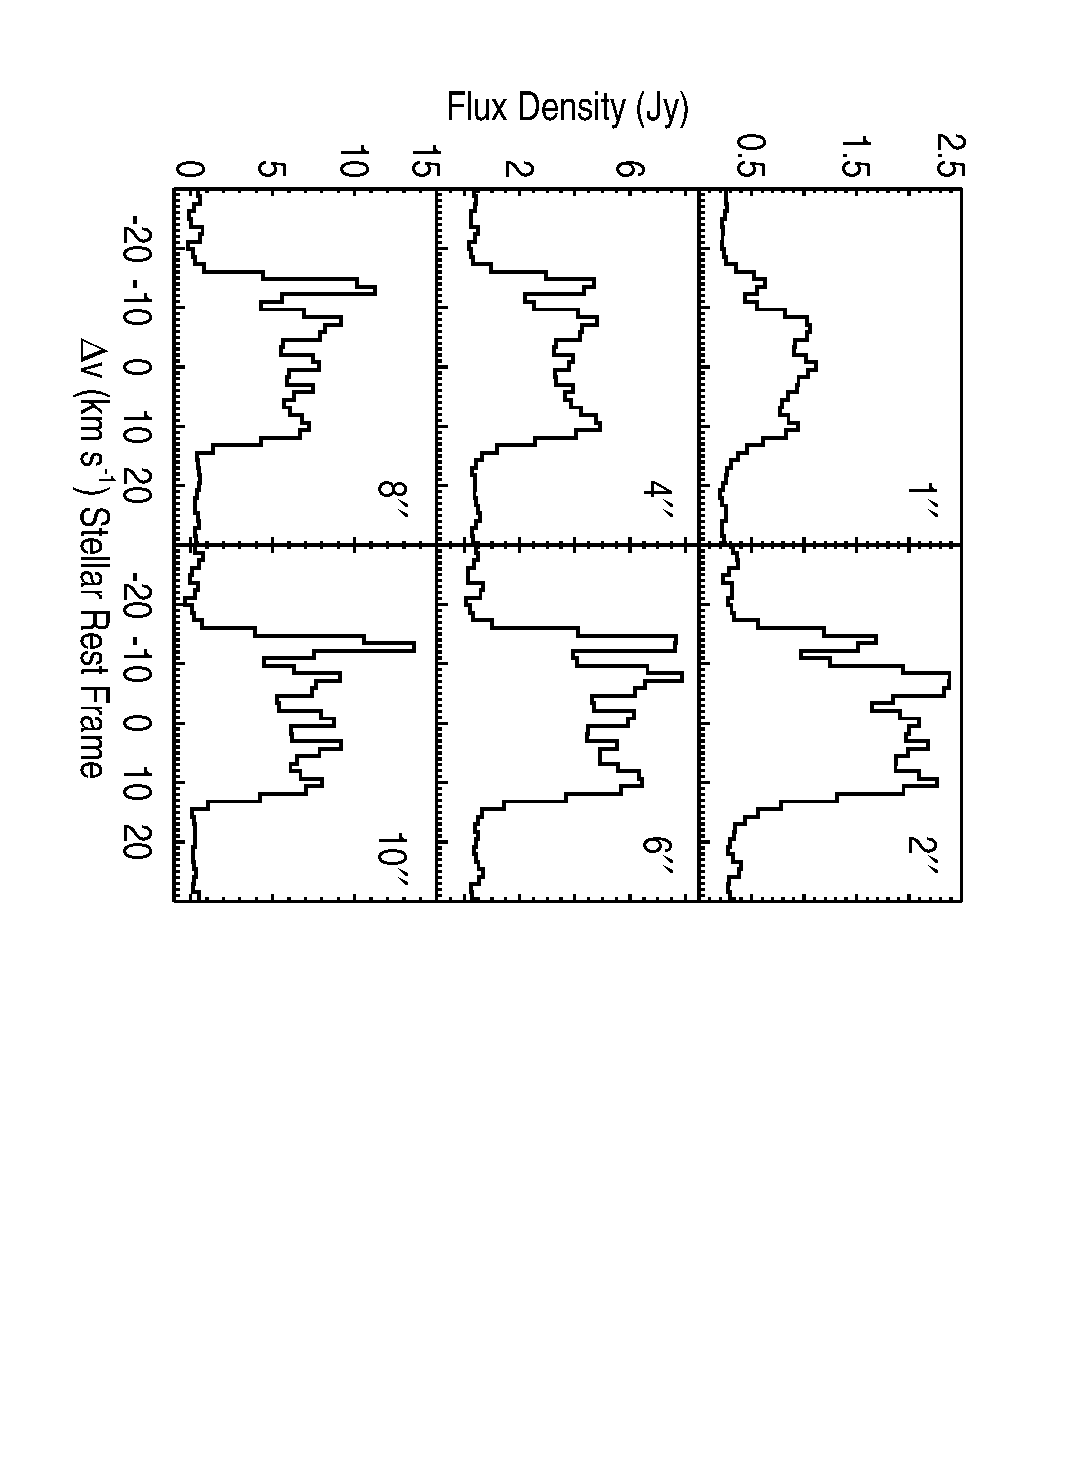
\includegraphics[scale=0.75, angle=90, width=13.0cm, height=11cm, trim=20pt 50pt 20pt 40pt]{test.eps}
\caption{Spectral profiles of the low spectral resolution multi-configuration image cube for circular extraction areas of radius 1$\arcsec$, 2$\arcsec$, 4$\arcsec$, 6$\arcsec$, 8$\arcsec$, and 10$\arcsec$.}
\label{fig:fig4}
\end{figure}

To obtain the most robust value for the S2 outflow velocities we examine the high resolution multi-configuration image cube spectrum which is composed of all tracks from all three configurations. It is worth stressing that by analyzing the multi-configuration image cube we make the crude assumption that the physical properties of all three components (i.e. $\alpha$ Ori, S1 shell and S2 shell) have not changed over the total observation period. The profile is found to have a total linewidth of 28.6 $\pm$ 0.7 km s${}^{-1}$, which is in close agreement with previous single dish observations of the line where values of 30.6 $\pm$ 2.5 km s${}^{-1}$ and 28.6 km s${}^{-1}$ are reported by \cite{1980ApJ...242L..25K} and \cite{1987ApJ...313..400H} respectively. The centroid velocity of the spectrum is  -1.1 km s${}^{-1}$ ($\rm{v_{lsr}}$ = 3.7 $\pm$ 0.7 km s${}^{-1}$) which is again in close agreement with \cite{1980ApJ...242L..25K} and \cite{1987ApJ...313..400H} who report values of 3.0 $\pm$ 2.5 km s${}^{-1}$ and 3.7 $\pm$ 0.4 km s${}^{-1}$ respectively. The integrated line flux is then 1.5 $\times 10^{-18}$ W m$^{-2}$ of which approximately 20\% emanates from the S1 shell.

The outflow velocities of the S2 shell are -15.4 km s${}^{-1}$ and +13.2 km s${}^{-1}$ which again like the S1 shell are slightly asymmetric but in the opposite sense. Note that these shell outflow velocities are dependent on the adopted radial velocity of Betelgeuse. If for instance, we instead adopt a radial velocity of 21.9 km s${}^{-1}$ \citep{2005A&A...430..165F} then the the S2 outflow velocities become even more asymmetric (-16.6 and +12.0 km s${}^{-1}$) while the S1 outflow becomes less so (-10.2 and +9.4 km s${}^{-1}$). Both shells therefore cannot have spherically symmetric outflow velocities regardless of the adopted stellar radial velocity. Adopting a mass of 18 M$_{\odot}$ and a radius of 950 R$_{\odot}$ \citep{2008AJ....135.1430H} then the escape velocity for Betelgeuse is 85 km s${}^{-1}$ which is much greater than the S1 and S2 shell outflow velocities. This indicates that the majority of the stellar mass loss mechanism's energy goes into lifting the CO molecules out of the gravitational potential and not into their outflow velocities. These outflow velocities are greater than the adiabatic hydrogen sound speed, which, if we assume that the gas temperature is the same as the excitation temperature, are 1.7 km s${}^{-1}$ and 1 km s${}^{-1}$ for the S1 and S2 shells respectively. 

The spectra in Figure 2 are taken from the low resolution multi-configuration image cube using circular extraction areas ranging in radius from 1$\arcsec$ to 10$\arcsec$ and demonstrates how the line profile changes over these different areas. The most striking change in the line profile is the change in appearance of the extreme blue wing. At small extraction radii where we sample the most compact emission, the feature is weak in comparison to the rest of the line but becomes more dominant as we begin to sample more of the extended emission. This indicates that even the high velocity components of the S2 shell have extended emission and this is why they are almost completely resolved out by CARMA's C configuration.

\subsection{Multi-Configuration Image Cube} \label{results2} 

A subset of the blueshifted velocity channel maps of the low spectral resolution multi-configuration image cube is presented in Figure \ref{fig:fig3}. The first channel map at -17.9 km s${}^{-1}$ shows just the compact unresolved continuum emission with no extended emission present. Between -16.7 km s${}^{-1}$ and -9.0 km s${}^{-1}$ we see evidence for the development of a classical shell signature for the S2 shell. We first sample the highest velocity shell components where the emission is relatively compact (i.e. between -16.7 km s${}^{-1}$ and -12.9 km s${}^{-1}$) and then sample lower velocity components where the shell becomes a faint ring (i.e. between -11.6 km s${}^{-1}$ and -9.0 km s${}^{-1}$). At lower velocities again, these rings disappear into the noise of the maps and possibly extend out beyond the primary beam at zero velocity when the rings should have maximum spatial extent. The emission from the channel maps between -15.3 km s${}^{-1}$ and -11.6 km s${}^{-1}$ correspond to all the emission in the extreme blue wing component of the multi-configuration image cube line profile discussed in \S3.1. We can see in Figure \ref{fig:fig3} that all of this emission is greater than the C configuration resolving out scale therefore confirming that our C configuration line profile is mainly composed of S1 shell emission. The shell formation signature of the S2 shell is also apparent in the redshifted velocity channel maps between +7.5 km s${}^{-1}$ and +13.8 km s${}^{-1}$ but the emission appears weaker and the rings fainter therefore indicating that the shell is inhomogeneous in density structure. 

\begin{figure}[hbt!]
%\centering
\mbox{
          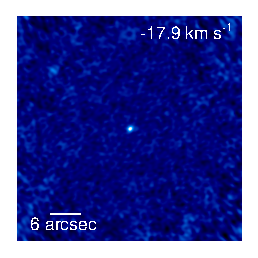
\includegraphics[]{chan41new.ps}
          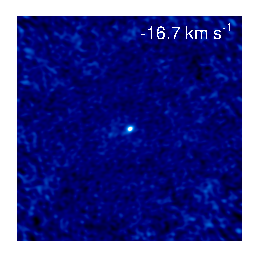
\includegraphics[]{chan40.ps}
          }
\\
\mbox{
          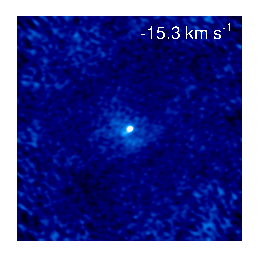
\includegraphics[]{chan39.ps}
          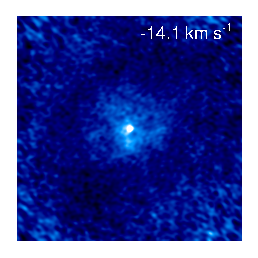
\includegraphics[]{chan38.ps}
          }
\\
\mbox{
          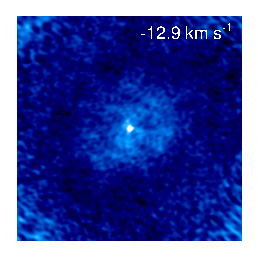
\includegraphics[]{chan37.ps}
          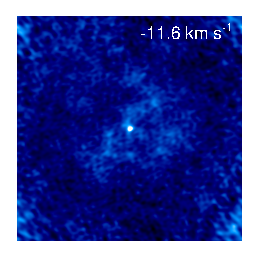
\includegraphics[]{chan36.ps}
         }
\\
\mbox{
          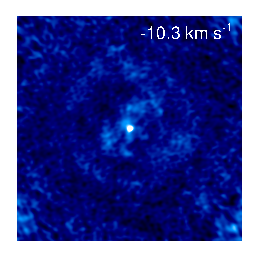
\includegraphics[]{chan35.ps}
          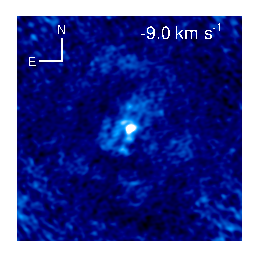
\includegraphics[]{chan34.ps}
         }
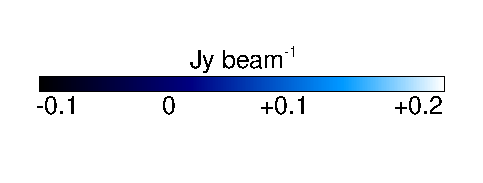
\includegraphics[trim=0pt 20pt 195pt 10pt]{color_bar.ps}
\caption{8 channel maps from the multi-configuration configuration image cube. The peak emission has been cut at 0.2 Jy beam${{}^{-1}}$ to emphasize the fainter emission. The color scale is linear and has been normalized to this maximum cutoff and minimum value of each channel. The emission at the corners of each map is a result of the primary beam correction.}
\label{fig:fig3}
\end{figure}

The multi-configuration maps also show the central compact emission from the S1 shell at velocities between -10.3 km s${}^{-1}$ and +11.3 km s${}^{-1}$. This S1 emission can be seen in the final two maps of Figure \ref{fig:fig3} as a central slightly elongated emission feature surrounded by the fainter rings of the S2 shell. In the maps where both shells are present the emission from the S1 shell appears brighter than the emission from the S2 shell. The spatial extent of the S1 shell varies from channel map to channel map and we assign it a mean radius of $\sim$ 5$\arcsec$, a value which in good agreement with \cite{2009AIPC.1094..868H} and \cite{2009AJ....137.3558S}. 

An additional spatially unresolved source is detected in a number of the D configuration image cube maps (both high and low spectral resolution) and has been previously documented by \citet{2009AIPC.1094..868H}. The component is present in only five continuous channels between $\sim$ -4 km s${}^{-1}$ and +2.4 km s${}^{-1}$ and is located $\sim$ 5$\arcsec$ S-W of $\alpha$ Ori as shown in Figure \ref{fig:fig2}. Its peak emission lies at $\sim$ 0 km s${}^{-1}$ and here it approximately equals 60$\%$ of the source peak emission. The corresponding channel maps in the E configuration image cube show extended emission out to ~8$\arcsec$ in the same S-W direction. This second source does not appear in any of the C configuration channel maps and may be resolved out by this extended configuration. This discrete second source thus has the effect of adding extra emission to the corresponding multi-configuration image cube maps at the low velocities where it is present.

\begin{figure}
\epsscale{1.0}
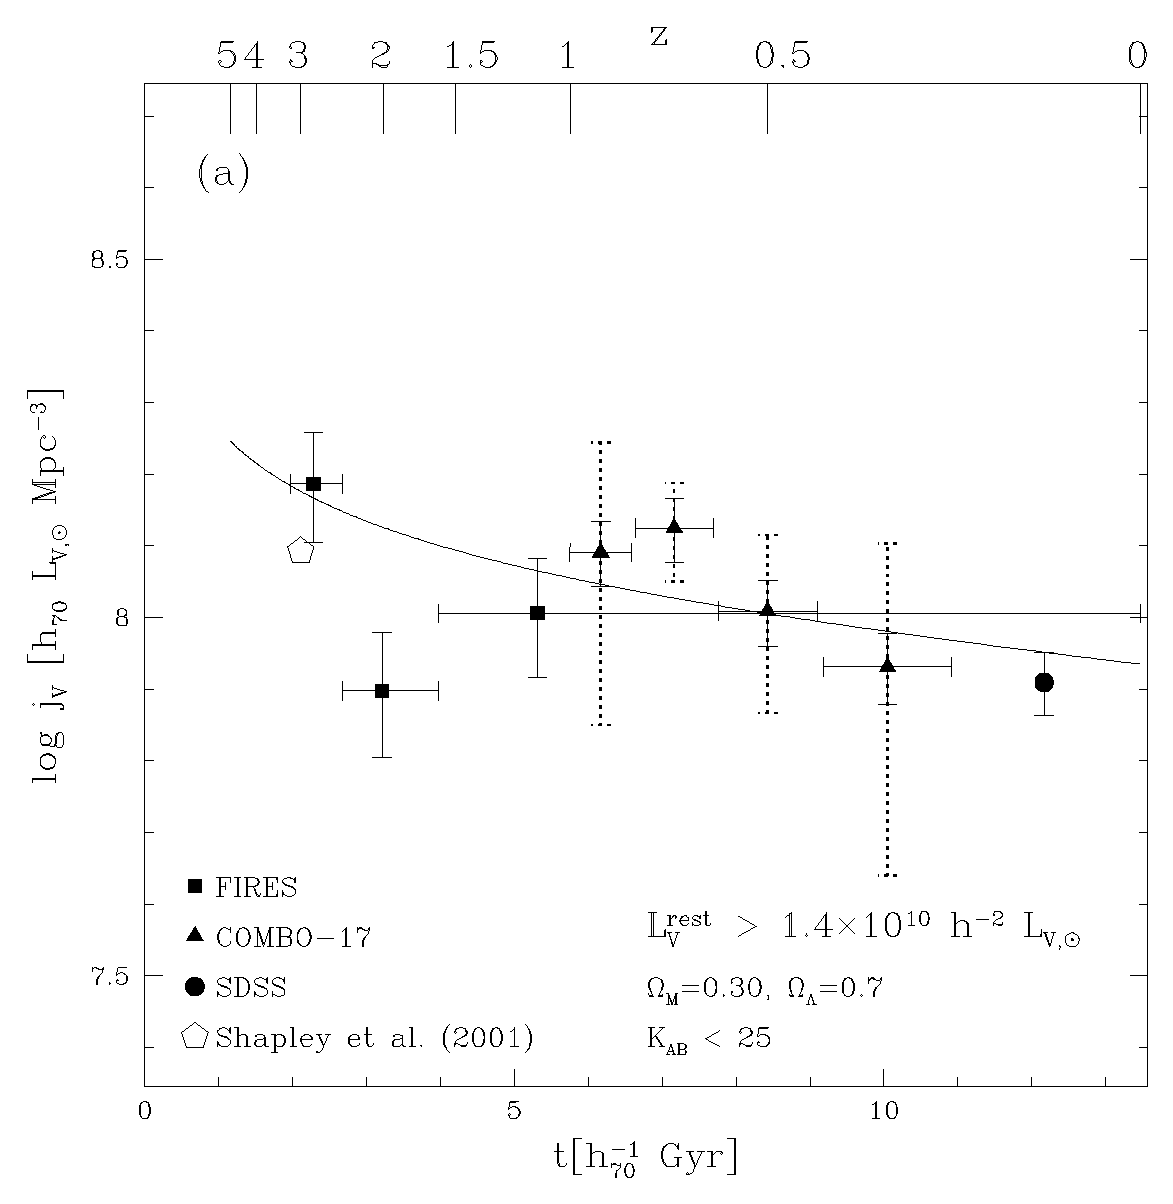
\includegraphics[trim=25pt 0pt 50pt 0pt, width=8.0cm, height=6.8cm]{f2.eps}
\caption{Integrated intensity image of the D configuration channel maps that contain the discrete second source approximately 5$\arcsec$ S-W of $\alpha$ Ori. Contours for the integrated intensity are 1$\sigma$, 1.5$\sigma$, 2$\sigma$, and 3$\sigma$ (1$\sigma$ = 1.3 Jy beam${}^{-1}$ km s${}^{-1}$). The size of the restoring beam is shown in white in the bottom left corner.}
\label{fig:fig2}
\end{figure}

\subsection{Determination of the Shell Radii} \label{results3} 
The spatial extent of the S1 and S2 shells around Betelgeuse was not directly determined from either the CO infrared absorption spectra of \cite{1979ApJ...233L.135B} or previous CO single dish radio observations \citep{1980ApJ...242L..25K, 1987ApJ...313..400H, 1994ApJ...424L.127H}. Our low spectral resolution multi-configuration image cube has sufficient spatial resolution and signal-to-noise to make direct estimates of the maximum radius of both shells. The outer S2 shell is not seen in the low absolute velocity channel maps where its spatial extent is maximum and either lies outside of the primary beam or is lost into the noise near the edge of the maps. We derive the maximum scale of the S2 shell by looking at the spatial scales of the S2 shell in the higher absolute velocity maps where the shell is present. If we assume that the S2 shell is spherically symmetric with a radius $R_{s}$, and is undergoing steady expansion with velocity $V_{s}$, then we can estimate the shell radius per velocity channel using the following relation:

\begin{equation}
\rm{r_{chan}}=R_{s} \rm{sin}\left[\rm{cos}^{-1}\left(\frac{v_{chan}}{V_{s}}\right) \right]
\end{equation} 
where $\rm{r_{chan}}$ is the shell radius in a channel at velocity $\rm{v_{chan}}$. 

We use Equation (1) to estimate the maximum projected spatial extent of the shell which occurs at zero velocity. An estimate of the S2 shell radius per channel ($\rm{r_{chan}}$) was found by creating annuli of increasing width around the central emission in each relevant line channel map of the multi-configuration image cube, extracting all flux within each annulus and then plotting these fluxes against distance from the star for each channel. The maximum of these resultant curves was then deemed to be the maximum radius of the S2 shell per channel. Figure 5 shows these data over-plotted with two model shells which were created using Equation (1). The blueshifted data points were best fitted by a model shell of maximum radius 17$\arcsec$ and outflow velocity 17 km s${}^{-1}$, while the redshifted data points were best fitted by a model shell of maximum radius 16$\arcsec$ and outflow velocity 14 km s${}^{-1}$. It is worth mentioning that this estimate for the spatial extent of the S2 shell is not dependent on our adopted radial velocity value for Betelgeuse and adopting a different radial velocity value would simply alter the shells outflow velocities. As the S2 shell is not present in our lowest absolute velocity map we are not able to report an estimate of the shell's width.

The S1 shell extends out to a mean distance of $\sim$ 5$\arcsec$ and is more extended in the S-W direction due to the presence of the second emission feature in the compact configuration data sets. The restoring beam size of 0.9$\arcsec$ is not sufficient to determine whether the S1 shell is discrete or an extension of the current wind phase seen in ultraviolet spectra, e.g., \citep{1997ApJ...479..970C}, and cm-radio continuum interferometry \citep{1998Natur.392..575L, harper_2001}.

\begin{figure}
\epsscale{1.2}
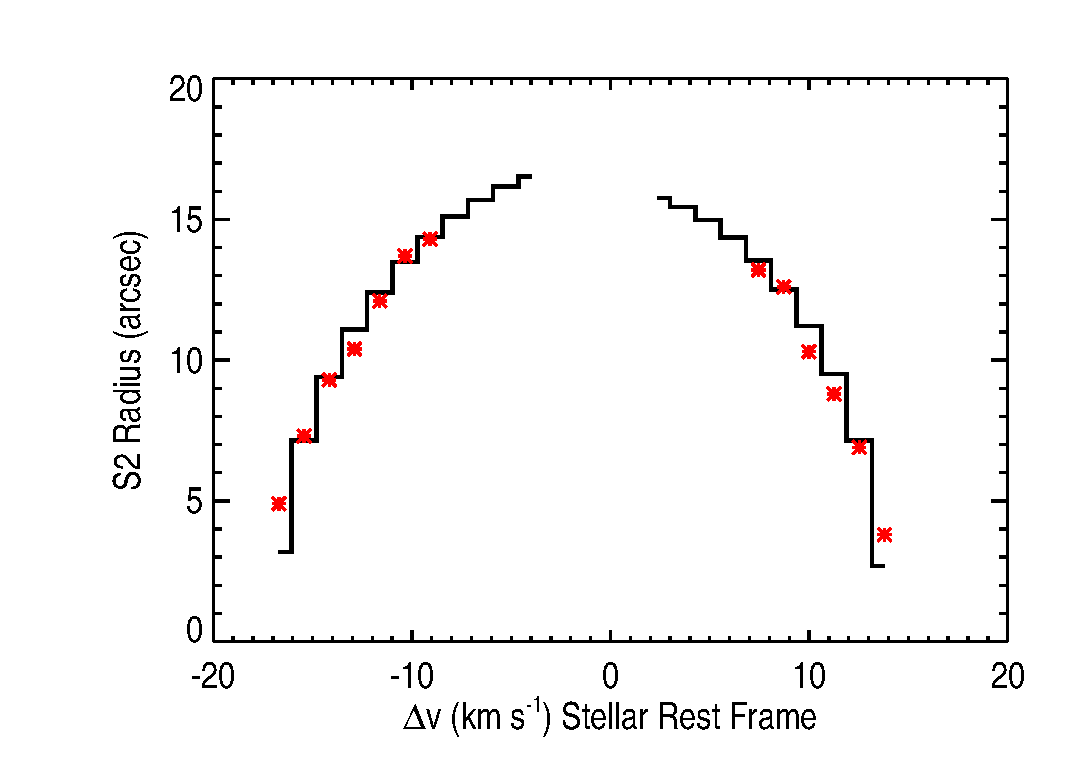
\includegraphics[trim=45pt 0pt 80pt 10pt, width=7.5cm, height=6.5cm]{s2_size.eps}
\caption{The derived shell radius as a function of velocity (red points) overplotted with two model shells. The blueshifted model (left) corresponds to a shell with a maximum radius of 17$\arcsec$ and an outflow velocity of 17 km s${}^{-1}$ while the redshifted model (right) corresponds to a shell with a maximum radius of 16$\arcsec$ and an outflow velocity of 14 km s${}^{-1}$.}
\label{fig:fig4}
\end{figure}
\
\
\subsection{Continuum Flux Densities} \label{results4} 

In Table 2 we show the derived continuum flux denities for each of the three configuration image cubes and also the multi-configuration image cube. The high spectral resolution ($\Delta v$ = 1.27 km s${}^{-1}$) image cubes were just wide enough to image the CO line but were too narrow to make accurate estimates of the continuum flux density. Therefore, all continuum flux density estimates are derived from the lower spectral resolution ($\Delta v$ = 0.635 km s${}^{-1}$) image cubes from which we were able to take accurate measurements at both sides of the line. We fitted elliptical Gaussians to $\sim$ 20 continuum channels using CASA's \textit{imfit} routine allowing the flux and corresponding uncertainties to be calculated. The source was unresolved in most of these continuum channels. 

Betelgeuse is known to show brightness variations at many wavelengths. \cite{1984PASP...96..366G} reports a decrease of half a magnitude in visual brightness over a period of six years. \cite{1987LNP...291..337B} found stochastic 30\%-40\% variations in flux density at 6 cm over timescales as short as 10 days to as long as 8 months (i.e. the observational period). A more comprehensive study was carried out by \cite{1992ASPC...26..455D} who observed Betelgeuse with the VLA at centimeter wavelengths from 1986 to 1990 and found stochastic variability of 22\%, 15\%, and 21\% at 6 cm, 3.6 cm, and 2 cm respectively at a variety of different timescales down to less than one month. The mm-continuum emission that we measure arises mainly from bremsstrahlung emission associated with neutral and ionized hydrogen and possibly dust emission, so it is not unreasonable to also expect variability at mm-wavelengths too. The D configuration data was acquired under adverse weather conditions and the data has the highest noise levels out of the three configurations. Its continuum emission measurement is approximately 50\% greater than the C and E configuration continuum measurements which were also acquired approximately two years after the D configuration data.  We believe the continuum emission derived from the multi-configuration image cube is an accurate estimation of the mm-continuum flux density over the two year period and is in reasonably good agreement with the 250 GHz flux density of \cite{1994A&A...281..161A} who report a value of 351$\pm$25 mJy.

\begin{deluxetable}{cccc}
\tabletypesize{\scriptsize}
\tablecaption{CARMA Continuum Fluxes}
\tablewidth{0pt}
\tablehead{
\colhead{Configuration} 		&
\colhead{Restoring Beam }		&
\colhead{Flux}			&
\colhead{Uncertainty}		\\
\colhead{}			&
\colhead{($\arcsec \times \arcsec$)}   	&
\colhead{(mJy)}			&
\colhead{(mJy)} 
}
\startdata
C & 0.96 $\times$ 0.76 & 234 & 18\\
D & 2.33 $\times$ 1.87 & 389 & 72\\
E & 4.93 $\times$ 3.84 & 278 & 40 \\
Multi-configuration & 1.05 $\times$ 0.84 & 289 & 21
\enddata
\label{tab:tab2}
\end{deluxetable}

\section{DISCUSSION}
\subsection{Previous CO Observations}
\cite{1979ApJ...233L.135B} were the first to detect circumstellar absorption lines in CO by looking at the 1-0 ro-vibration line at 4.6 $\mu$m. These infrared observations revealed two shells around $\alpha$ Ori; a warm (\rm{$T_{exc}$} = 200 K) S1 shell with an expansion velocity of 9 km s${}^{-1}$ and a cooler (\rm{$T_{exc}$} = 70 K) S2 shell moving with a faster expansion velocity of 16 km s${}^{-1}$.   \cite{1980ApJ...242L..25K} were the first to detect emission in the CO($J=$ 2-1) line at 1.3 mm using the 10 m millimeter-wave telescope at Owens Valley Radio Observatory but only detected one component expanding at 15 km s${}^{-1}$. By reconciling column densities, they concluded that the shell radii derived by \cite{1979ApJ...233L.135B} were too large and that S2 lies at a radius of R $\leq$ 10$\arcsec$. Since the detection by Knapp, a number of follow up observations at 1.3 mm have been carried out with various beam sizes and all spectra look remarkably similar; that is the profile has a steep extreme blue shifted emission component with the remainder of the profile looking more flat topped and containing a number of less dominant spikes. \cite{1987ApJ...313..400H} used their single dish observations (beam size $\sim$ 32$\arcsec$) of the CO($J=$ 2-1) line along with excitation and self-shielding models of CO to conclude that the S1 shell makes little contribution to the final emission line. They also identify the extreme blue wing of the line with the S2 shell and predict that it may extend out to a radius of $\sim$ 16$\arcsec$. Later however, \cite{1994ApJ...424L.127H} compared their detected 609 $\mu$m ${}^3P{}_1\rightarrow{}^3P{}_0$ fine structure line of C I with CO data obtained with the IRAM 30m telescope (beam size $\sim$ 12$\arcsec$) and find that the expansion velocities in both lines are essentially the same. They conclude that the radial extent of C I is $\lesssim$ 7$\arcsec$ and both the CO and C I are formed in the inner envelope and roughly extend over the same area.  

The shape of our multi-configuration line profile for extraction areas of radii 6$\arcsec$ or greater are in good agreement with previous high signal to noise single dish CO($J=$ 2-1) spectra \cite[e.g.][Fig. 1.]{1994ApJ...424L.127H} although the emission spikes in our line profiles are more dominant. Our total line width of 28.6 km s${}^{-1}$ is in good agreement with \cite{1987ApJ...313..400H} and \cite{1994ApJ...424L.127H} who report line widths of 28.6 km s${}^{-1}$ and 30 km s${}^{-1}$ respectively. The extreme blue wing in both of these spectra are the dominant emission features of the line and this is also true in our multi-configuration spectra at extraction areas $\gtrsim$ 6$\arcsec$. The IRAM 30 m telescope in \cite{1994ApJ...424L.127H} has a beam size of only 12$\arcsec$ at 230 GHz and yet produces a similar line profile shape to \cite{1987ApJ...313..400H} who uses a larger beam size of $\sim$30$\arcsec$. From this, one would expect that the majority of the blue wing emission is compact. Our multi-configuration line profiles suggest otherwise however, and show a continuous increase in the blue wing emission as we take larger extraction regions out to 10$\arcsec$. The multi-configuration maps also show a faint ring structure forming at $\sim$ 11.6 km s${}^{-1}$ and expanding further out as we sample across the channels. This ring emission is fainter than the higher velocity compact emission so we see a drop in flux density in our spectra at the point where these rings form. Therefore, the steepness of the extreme blue wing in our multi-configuration spectrum does not actually mean that we are resolving the S2 shell but merely that there is more CO emitting at higher velocities than at lower.

The line profiles of higher CO rotational transitions for Betelgeuse have been published in \cite{2003A&A...407..609K} and \cite{2010A&A...523A..18D}. \cite{2010A&A...523A..18D} present high spectral resolution (0.3125 MHz) line profiles for the CO($J=$ 2-1), ($J=$ 3-2), and ($J=$ 4-3) transitions that were obtained with the James Clerk Maxwell Telescope (JCMT). For the CO($J=$ 2-1) transition the JCMT has a HPBW of $\sim$ 20$\arcsec$ and the profile appears similar to our multi-configuration profile over the same flux density extraction area (i.e. Figure 2), with the extreme blue wing component being the dominant feature in both. This feature, which is emission from the S2 shell becomes a less dominant component of the line profile at the higher CO($J=$ 3-2) and CO($J=$ 4-3) transitions where the JCMT has a HPBW of $\sim$ 13$\arcsec$ and 8$\arcsec$ respectively, and does not capture all of the S2 emission which is shown in Figure 3 to be extended at these velocities. We expect this trend in the change of the profile shape to continue at higher rotational transitions again where the HPBW would be smaller thus capturing even less of the S2 emission. Also the probability of these high rotational states being occupied would become increasingly less (assuming an S2 excitation temperature of 70 K) and therefore the profile would become dominated by emission from the S1 shell with it's higher excitation temperature ($\sim$ 200 K).

The CO 4.6 $\mu$m vibration-rotational lines have been observed with the Phoenix spectrograph \citep{1998SPIE.3354..810H} by \cite{1999A&A...347L..35R} and \cite{2009AJ....137.3558S} on the 2.1 m telescope at Kitt Peak and on the 8.1 m Gemini South telescope respectively. By assuming a Boltzmann population distribution for the ground rotational levels of CO \cite{1999A&A...347L..35R}  derived a mean excitation temperature of 38${}^{+6}_{-5}$ K along the line of sight at a projected distance of 4$\arcsec$ north of Betelgeuse with a slit length of 50$\arcsec$. Our CARMA data suggests that the S1 shell extends out beyond this but Ryde et al.'s temperature is not in agreement with either of the line-of-sight S1 or S2 excitation temperatures of 200${}^{+50}_{-10}$\,K and 70$\pm 10$\,K derived by \cite{1979ApJ...233L.135B}. This discrepancy may indicate the excitation is quite non-uniform.
\cite{2009AJ....137.3558S} did not derive an excitation temperatures but used their 4.6 $\mu$m spectra to reveal extended resonantly scattered CO emission out to $\sim$ 3 - 5$\arcsec$ in good agreement with our mean S1 radial value. They observe emission over a velocity range of 30 km s${}^{-1}$ but two distinct shells are not detected. Mild ($\sim$ 20\%) density inhomogenities are reported but overall, their observations are consistent with a spherical, optically thin and steady wind.

\subsection{K I 7699 \AA \ spectra}

The S2 shell was first identified in high resolution K~I and Na~I absorption spectra by \cite{1975ApJ...199..427G} and subsequently re-observed multiple times over the next couple of years \citep{1979QJRAS..20..361G}. It is interesting to compare these line-of-sight velocities with those from the CARMA emission spectra obtained at similar spectral resolutions.

We have obtained K I 7698.98 \AA \ spectra using the cross-dispersed echelle spectrometers on the Harlan J. Smith 107 inch (2.7m) reflector at McDonald Observatory. With two pixels per resolution element a $R=\lambda/\Delta\lambda=200,000$ and a $R=500,000$ spectrum were obtained in 2007 March 25 and April 13, universal time, respectively. The spectra were wavelength calibrated with ThAr lamp lines and the lower resolution spectrum was checked by fitting six symmetric terrestrial O${}_2$ lines in the same order using wavelengths from \cite{1948ApJ...108..167B}. The O${}_2$ lines confirmed the R=200,000 calibration was good to better than $0.1\>{\rm km\>s}^{-1}$. Upon cross-correlating the low and high resolution spectrum the high resolution spectrum appeared redshifted by $0.60\>{\rm km\>s}^{-1}$, i.e., one resolution element, for which we do not have an explanation except to note that a similar offset has been reported by \cite{1994ApJ...436..152W}. We use the cross-correlation to define the wavelength calibration of the $R=500,000$ spectrum and we adopt a systematic error of $0.2\>{\rm km\>s}^{-1}$.

\begin{figure}
\epsscale{1.0}
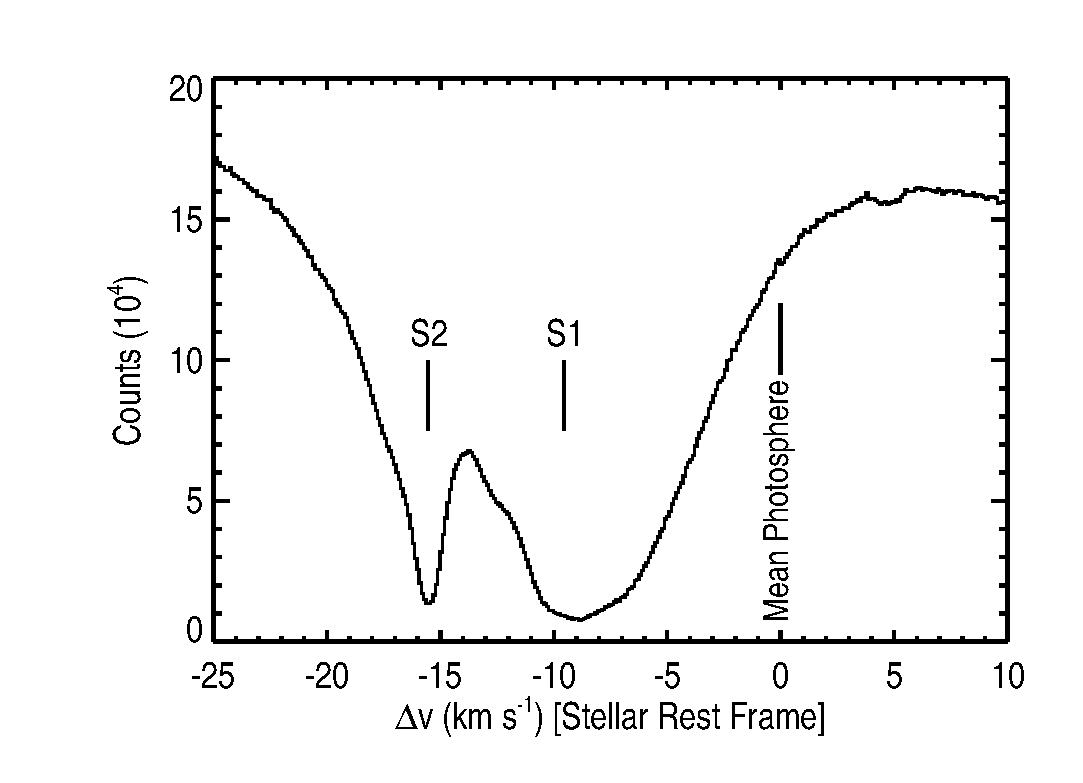
\includegraphics[trim=40pt 0pt 50pt 0pt, width=8.0cm, height=7.5cm]{macdon.eps}
\caption{The K~I 7698.98 \AA \  profile (R=500,000) for Betelgeuse obtained on April 13th 2007. The S2 shell outflow velocity is found to be 15.6 km s${}^{-1}$ (using a V$_{rad}$ = +20.7 km s${}^{-1}$), slightly lower than \citeauthor{2002A&A...386.1009P}'s \citeyearpar{2002A&A...386.1009P} value of 18$\pm$2 km s${}^{-1}$.}
\label{fig:fig5}
\end{figure}

The high-resolution spectrum is shown in Figure 6 in the adopted stellar centre-of-mass rest frame ($V_{rad}=+20.7\>{\rm km\>s}^{-1}$). The S2 feature is deep, well separated from the S1 feature, and very well represented by a simple absorption model with hyperfine splitting. We adopt the K~I $7698.9645$ $\rm{\AA}$ line parameters compiled in \cite{2003ApJS..149..205M}\footnote{Note that this wavelength is $0.44\>{\rm km\>s}^{-1}$ less that that adopted in the Goldberg studies.} and find a heliocentric S2 absorption velocity of $+5.1\>{\rm km\>s}^{-1}$ and a most probable line-of-sight turbulent velocity of $0.60\>{\rm km\>s}^{-1}$. There is also a slight inflection in the underlying profile at $+3.6\>{\rm km\>s}^{-1}$ (heliocentric) which may represent structure in the underlying photospheric profile or additional absorption in which case it has $\sim 0.1$ the column density of S2.  The S2 absorption minimum can be compared to those obtained by \citet[Fig 7]{1979QJRAS..20..361G} who measured values between 1975 and 1978 of $4.2\pm 0.2$ and $5.0\pm 0.2 \>{\rm km\>s}^{-1}$ and these differences may result from changes caused by radial velocity changes in the underlying photospheric spectrum. Bernat et al.'s 1979 CO IR absorption observations reveal S2 heliocentric velocities of $+4.94\pm 0.30$ $\>{\rm km\>s}^{-1}$ (1979 Mar 6) and $+4.60\pm 0.04$ \>{\rm km\>s}^{-1}$ (1979 Apr 14) with turbulent velocities of 4 and $1\>{\rm km\>s}^{-1}$ for the S1 and S2 features, respectively.

In terms of the center-of-mass radial velocity of the star our K~I feature implies an outflow velocity of $+15.6\>{\rm km\>s}^{-1}$. The blue edge of our CARMA multi-configuration CO profile is estimated to be $+15.4\>{\rm km\>s}^{-1}$  which suggests a dynamical association with the CO S2 shell and very close agreement with \citeauthor{1979ApJ...233L.135B}'s \citeyearpar{1979ApJ...233L.135B} CO absorption velocities listed above. \cite{2002A&A...386.1009P} have also estimated the radius and velocity of the suspected K~I S2 shell using $R=110,000$ resolution long slit spectra. They found a geometrically thin shell (1$\arcsec$) with velocity of $V_{S2}=18\pm 2\>{\rm km\>s}^{-1}$ with a radius of 55$\arcsec$ which is much larger than the field of view of the CARMA spectra. Their long slit spectra show several smaller partial shells but it is not simple to directly associate the CO emission feature with one or more of these shells especially given the uncertainty in the ionization balances of CO and K~I.

\section{CONCLUSIONS}
%\textcolor{red}{}
The two distinct velocity components seen by \cite{1979ApJ...233L.135B} in CO absorption against the stellar spectrum at 4.6 $\mu$m have both been detected at 230 GHz for the first time. The first velocity component known as S1 has an expansion velocity of 9 km s${}^{-1}$ \citep{1979ApJ...233L.135B} and is detected in our high spectral resolution C configuration profile with the same blueshifted velocity (i.e. 9.0 km s${}^{-1}$) and with a larger redshifted outflow velocity of 10.6 km s${}^{-1}$. The extended CARMA C configuration has a resolving out scale of $\sim$ 6 $\arcsec$ and thus resolves out almost all of the S2 emission leaving us with an approximate spectrum for the S1 shell. An extreme blue wing of the CO spectrum appears in the D and E configuration spectra which we associate with the S2 shell. The high spectral resolution multi-configuration spectrum is used to determine S2 outflow velocities of -15.4 km s${}^{-1}$ and +13.2 km s${}^{-1}$ which is in good agreement with our K I 7699 \AA \ line of sight S2 velocity and that reported by \cite{1979ApJ...233L.135B}. 

Our derived S1 radius is in good agreement with the the Phoenix measurements of \cite{2009AJ....137.3558S} and our high spatial resolution multi-configuration maps provide the first direct measurements on the spatial extent of the S2 shell, which we derive to have a radius of 17$\arcsec$; a value that higher than most previous estimates. Previous single dish observations of the CO line with small HPBWs do not show the classical resolved  signature of high emission at large absolute velocities and low emission at low absolute velocities for two main reasons. Firstly, the S1 shell is still unresolved in these single dish observations and thus contributes emission and at the lower absolute velocities. As well as this, the multi-configuration CARMA maps show that the S2 shell emission is brighter in the higher absolute velocity maps than at lower absolute velocities and so when the emission from the fainter rings is neglected (i.e. when they are resolved), the overall line profile does not change significantly. Assuming a mean constant outflow velocity of 14.3 km s${}^{-1}$ and 9.8 km s${}^{-1}$ for the S2 and S1 shell respectively then their ages are $\sim$ 1100 yr and $\sim$ 470 yr. 

\acknowledgments

Support for CARMA construction was derived from the states of California, Illinois, and
Maryland, the James S. McDonnell Foundation, the Gordon and Betty Moore Foundation, the
Kenneth T. and Eileen L. Norris Foundation, the University of Chicago, the Associates of the
California Institute of Technology, and the National Science Foundation. Ongoing CARMA
development and operations are supported by the National Science Foundation under a
cooperative agreement, and by the CARMA partner universities.

Based [in part] on observations made with the NASA/DLR Stratospheric Observatory for Infrared Astronomy. SOFIA Science Mission Operations are conducted jointly by the Universities Space Research Association, Inc., under NASA contract NAS2-97001, and the Deutsches SOFIA Institut under DLR contract 50 OK 0901. GREAT is a development by the MPI für Radioastronomie and the KOSMA/ Universität zu Köln, in cooperation with the MPI für Sonnensystemforschung and the DLR Institut für Planetenforschung.

{\it Facilities:} \facility{CARMA}, \facility{McDonald Observatory} and \facility{SOFIA}.

\appendix

\section{SOFIA OBSERVATIONS}

\bibliography{references}
\begin{figure}
\epsscale{1.0}
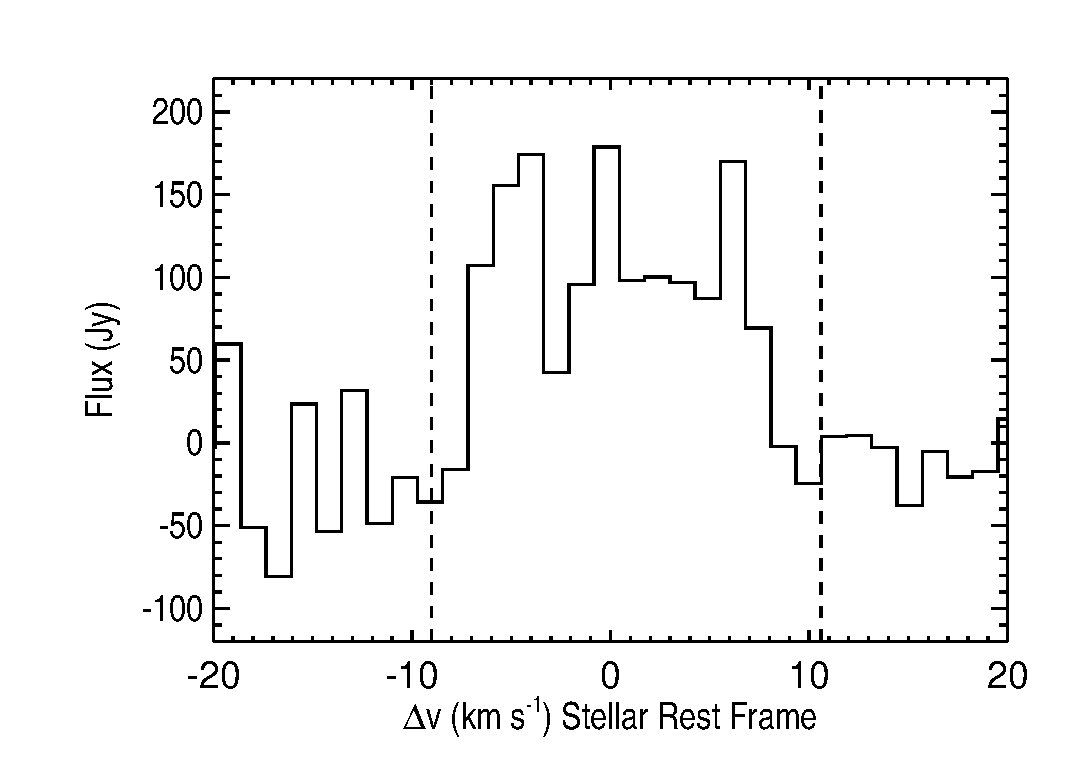
\includegraphics[trim=40pt 0pt 50pt 0pt, width=8.0cm, height=7.5cm]{sofia_spec_aj.eps}
\caption{}
\label{fig:fig6}
\end{figure}
\end{document}